\section{Analysis}

\subsection{Use Case analysis}

\subsubsection{Class Candidates}
In order to find potential class candidates, every noun of the detailed Use
Cases are found. These are potential candidates, and can be sorted to avoid
duplicates and candidates that won’t be turned into classes. Naturally, every
potential class for the entire system will not be found, as this only reflects
use cases. A potential class candidate such as MES (where Start and Stop
functionality would otherwise be implemented) will not be reduced to a single
class and is therefore not added to the list of class candidates.

The final list of classes, as well as a description of them, can be seen in
table \ref{table:class_candidates}.

\begin{table}[ht]
    \begin{tabularx}{\textwidth}{|>{\RaggedRight}p{4cm}|>{\RaggedRight}p{6cm}|>{\RaggedRight}X|}
    \hline
    \textbf{Class Candidate} & \textbf{Attributes}                                                                                                     & \textbf{Definition}                                                                    \\ \hline
    Batch                    & Id, type, product\_amount (total, defect, acceptable), amount (time), state (current, history), OEE, production\_speed, & A batch refers to a specific batch of products the brewery has made                    \\ \hline
    Product                  & Id, type, Ingredients,                                                                                                  & Product refers to the different options of beer to be produced                         \\ \hline
    Ingredient               & Name, id                                                                                                                & An ingredient refers to a specific ingredient. Products contain a list of ingredients. \\ \hline
    \end{tabularx}
    \caption{Potential class candidates}
    \label{table:class_candidates}
    \end{table}

\subsubsection{UML Analysis Diagram}
From the verb/noun analysis from the previous chapter, the UML analysis diagram
seen in figure \ref{figure:analysis_diagram}, can be generated. This diagram
shows the classes and attributes found in the requirements from the project
description.

\begin{figure}[ht]
	\centering 
	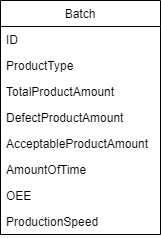
\includegraphics[scale=0.6]{images/diagrams/UML_Analysis_Diagram.drawio.png}
	\caption{UML Analysis diagram}
	\label{figure:analysis_diagram} 
\end{figure}

\subsection{Use Case Realisation}

\subsubsection{Sequence Diagrams}

            % \begin{enumerate}
            %     \item A beer type should be selected
            % \end{enumerate}

\subsubsection{Operation Contracts}
An operation contract describes the responsibility of the operation. 
The contract focuses on what the operation can change, and not how it is changed. 
It is also used to describes the state of the system before and after the 
operation is called.
\begin{table}[H]
    \begin{tabularx}{\textwidth}{|>{\RaggedRight}p{3.7cm}|>{\RaggedRight}X|}
        \hline
        \multicolumn{2}{|c|}{\textbf{start}}\\
        \hline
        \textbf{System operation} & start\\
        \hline
        \textbf{Cross References} & Use case: Start machine see table \ref{table:usecase_start} \\
        \hline
        \textbf{Responsibility} & Starting the beer machine if the pre-conditions 
        is met.
            If the pre-conditions is not met, the beer machine will not start \\
        \hline
        \textbf{Output} & The beer machine started the production\\
        \hline
        \textbf{Pre-conditions} & 
            The beer production machine needs to be in
            ready mode, that is, not producing beer. \\
        \hline
        \textbf{Post-conditions} & The beer machine started brewing\\
        \hline
    \end{tabularx}
    \caption{Operation Contracts start} 
    \label{table:Operation_Contracts_start}
\end{table}

\begin{table}[H]
    \begin{tabularx}{\textwidth}{|>{\RaggedRight}p{3.7cm}|>{\RaggedRight}X|}
        \hline
        \multicolumn{2}{|c|}{\textbf{stopProduction}}\\
        \hline
        \textbf{System operation} & stopProduction\\
        \hline
        \textbf{Cross References} & Use case: Stop the beer Machine see table \ref{table:usecase_stop}\\
        \hline
        \textbf{Responsibility} & Stop's the beer machine if the pre-conditions is met.
        If the pre-conditions is not met, the beer machine will not do anything\\
        \hline
        \textbf{Output} & The beer machine is stopped\\
        \hline
        \textbf{Pre-conditions} & The beer machine needs to be running\\
        \hline
        \textbf{Post-conditions} & The beer machine is stopped\\
        \hline
    \end{tabularx}
    \caption{Operation Contracts stopProduction} 
    \label{table:Operation_Contracts_stopProduction}
\end{table}


\begin{table}[H]
    \begin{tabularx}{\textwidth}{|>{\RaggedRight}p{3.7cm}|>{\RaggedRight}X|}
        \hline
        \multicolumn{2}{|c|}{\textbf{reset}}\\
        \hline
        \textbf{System operation} & reset \\
        \hline
        \textbf{Cross References} & Use case: reset see table \ref{table:usecase_reset} \\
        \hline
        \textbf{Responsibility} & It is responsible for resetting the beer 
                machine.\\
        \hline
        \textbf{Output} & reset the beer machine. \\
        \hline
        \textbf{Pre-conditions} & The beer production machine needs to be in
                ready mode, that is, not producing beer. \\
        \hline
        \textbf{Post-conditions} & The beer production machine has been reset. \\
        \hline
    \end{tabularx}
    \caption{Operation Contracts reset} 
    \label{table:Operation_Contracts_reset}
\end{table}

\begin{table}[H]
    \begin{tabularx}{\textwidth}{|>{\RaggedRight}p{3.7cm}|>{\RaggedRight}X|}
        \hline
        \multicolumn{2}{|c|}{\textbf{clear}}\\
        \hline
        \textbf{System operation} & clear\\
        \hline
        \textbf{Cross References} & Use case: clear see table \ref{table:usecase_reset} \\
        \hline
        \textbf{Responsibility} & It is responsible for clearing the beer 
                machine. \\
        \hline
        \textbf{Output} & The beer machine has been cleared. \\
        \hline
        \textbf{Pre-conditions} & The beer production machine needs to be in
                ready mode, that is, not producing beer. \\
        \hline
        \textbf{Post-conditions} & The beer production machine has been cleared.\\
        \hline
    \end{tabularx}
    \caption{Operation Contracts clear} 
    \label{table:Operation_Contracts_clear}
\end{table}

\begin{table}[H]
    \begin{tabularx}{\textwidth}{|>{\RaggedRight}p{3.7cm}|>{\RaggedRight}X|}
        \hline
        \multicolumn{2}{|c|}{\textbf{display live data}}\\
        \hline
        \textbf{System operation} & displayLiveData\\
        \hline
        \textbf{Cross References} & Use case: displayLiveData see table \ref{table:usecase_displayLiveData} \\
        \hline
        \textbf{Responsibility} & It is responsible for posting data to the client. \\ 
        \hline
        \textbf{Output} & Post data to the client.  \\
        \hline
        \textbf{Pre-conditions} & The beer production machine needs to be on and
                producing beer. \\
        \hline
        \textbf{Post-conditions} & Live data has been displayed for the user. \\
        \hline
    \end{tabularx}
    \caption{Operation Contracts monitorAndDisplayData} 
    \label{table:Operation_Contracts_monitorAndDisplayData}
\end{table}

\begin{table}[H]
    \begin{tabularx}{\textwidth}{|>{\RaggedRight}p{3.7cm}|>{\RaggedRight}X|}
        \hline
        \multicolumn{2}{|c|}{\textbf{batchReport}}\\
        \hline
        \textbf{System operation} & batchReport\\
        \hline
        \textbf{Cross References} & Use case: batchReport see table \ref{table:usecase_batchReport} \\
        \hline
        \textbf{Responsibility} &  Make a report after the pre-conditions is met
                and adds the report to the database.\\
        \hline
        \textbf{Output} & Produces a batch report and display it for the user.\\
        \hline
        \textbf{Pre-conditions} & The beer Machine needs to have produced a batch.\\
        \hline
        \textbf{Post-conditions} & A batch report has been displayed for the
                user. \\
        \hline
    \end{tabularx}
    \caption{Operation Contracts produceBatchReport} 
    \label{table:Operation_Contracts_produceBatchReport}
\end{table}

\subsubsection{Updated UML Class Diagram}
